\documentclass{standalone}
\usepackage{tikz}
\usetikzlibrary{patterns, positioning}

\begin{document}
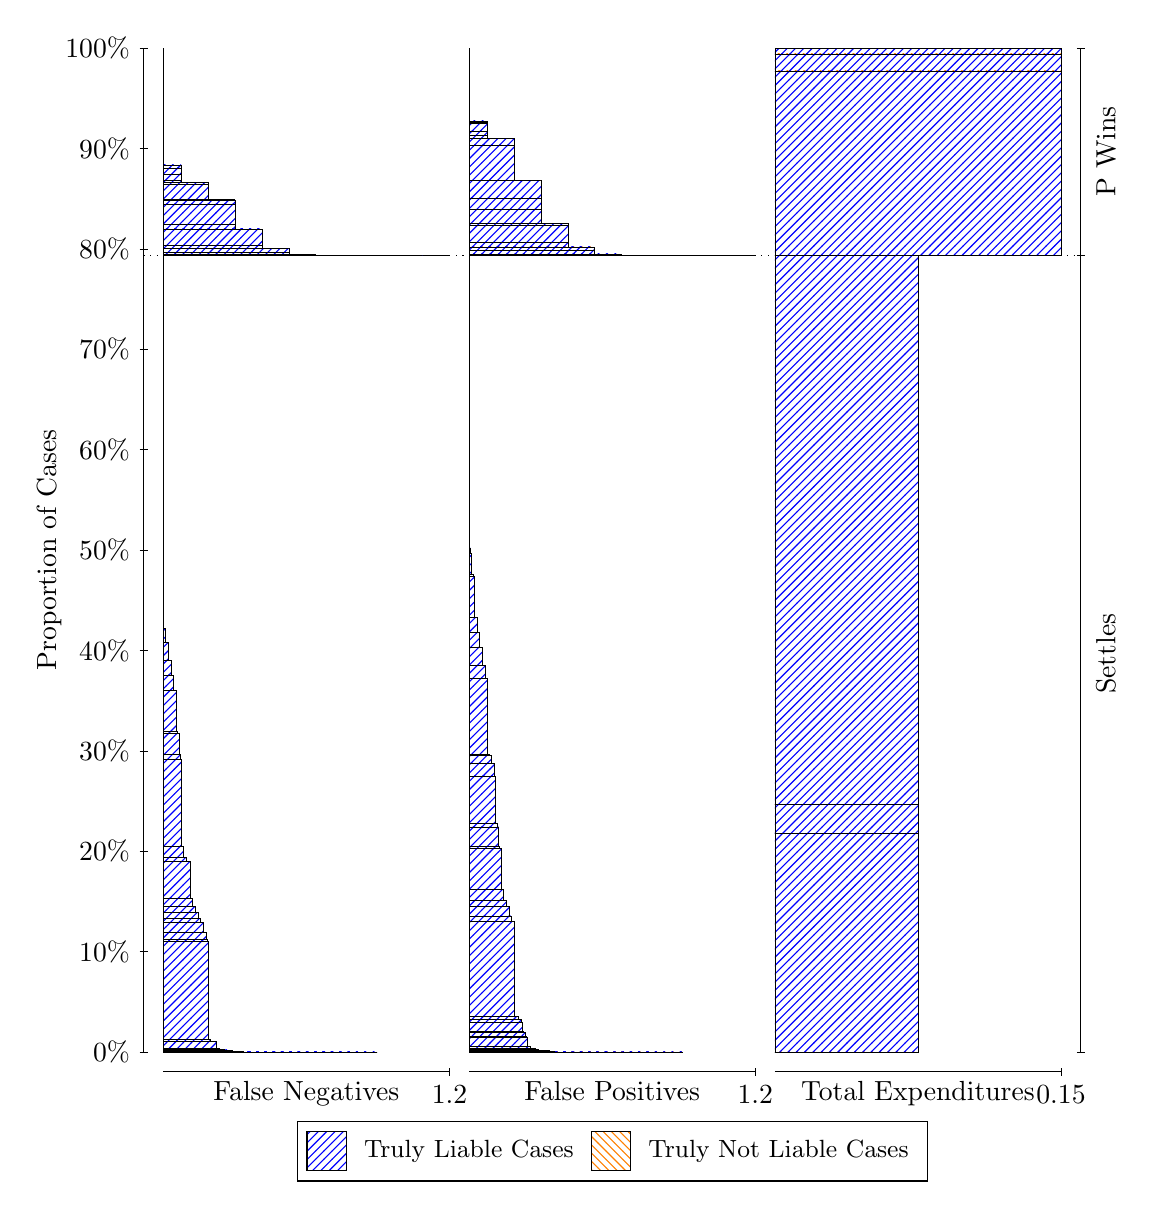
\begin{tikzpicture}
\draw[black, very thin] (1.5,1.75) -- (1.5,14.5);
\node[rotate=90, anchor=center] at (0.3, 8.125) {Proportion of Cases};
\draw[black, very thin] (1.45,1.75) -- (1.55,1.75);
\node[anchor=east] at (1.45, 1.75) {0\%};
\draw[black, very thin] (1.45,3.025) -- (1.55,3.025);
\node[anchor=east] at (1.45, 3.025) {10\%};
\draw[black, very thin] (1.45,4.3) -- (1.55,4.3);
\node[anchor=east] at (1.45, 4.3) {20\%};
\draw[black, very thin] (1.45,5.575) -- (1.55,5.575);
\node[anchor=east] at (1.45, 5.575) {30\%};
\draw[black, very thin] (1.45,6.85) -- (1.55,6.85);
\node[anchor=east] at (1.45, 6.85) {40\%};
\draw[black, very thin] (1.45,8.125) -- (1.55,8.125);
\node[anchor=east] at (1.45, 8.125) {50\%};
\draw[black, very thin] (1.45,9.4) -- (1.55,9.4);
\node[anchor=east] at (1.45, 9.4) {60\%};
\draw[black, very thin] (1.45,10.675) -- (1.55,10.675);
\node[anchor=east] at (1.45, 10.675) {70\%};
\draw[black, very thin] (1.45,11.95) -- (1.55,11.95);
\node[anchor=east] at (1.45, 11.95) {80\%};
\draw[black, very thin] (1.45,13.225) -- (1.55,13.225);
\node[anchor=east] at (1.45, 13.225) {90\%};
\draw[black, very thin] (1.45,14.5) -- (1.55,14.5);
\node[anchor=east] at (1.45, 14.5) {100\%};

\draw[black, very thin] (13.4,1.75) -- (13.4,14.5);
\draw[black, very thin] (13.35,1.75) -- (13.45,1.75);
\node[anchor=west] at (13.35, 1.75) {};
\draw[black, very thin] (13.35,11.866) -- (13.45,11.866);
\node[anchor=west] at (13.35, 11.866) {};
\draw[black, very thin] (13.35,14.5) -- (13.45,14.5);
\node[anchor=west] at (13.35, 14.5) {};

\draw[black, very thin, pattern color=blue, pattern=north east lines] (1.75,1.75) rectangle (4.4654,1.75);
\draw[black, very thin, pattern color=blue, pattern=north east lines] (1.75,1.75) rectangle (4.3125,1.75);
\draw[black, very thin, pattern color=blue, pattern=north east lines] (1.75,1.75) rectangle (4.1595,1.75);
\draw[black, very thin, pattern color=blue, pattern=north east lines] (1.75,1.75) rectangle (4.1255,1.75);
\draw[black, very thin, pattern color=blue, pattern=north east lines] (1.75,1.75) rectangle (4.0065,1.75);
\draw[black, very thin, pattern color=blue, pattern=north east lines] (1.75,1.75) rectangle (3.9725,1.75);
\draw[black, very thin, pattern color=blue, pattern=north east lines] (1.75,1.75) rectangle (3.8535,1.75);
\draw[black, very thin, pattern color=blue, pattern=north east lines] (1.75,1.75) rectangle (3.8195,1.75);
\draw[black, very thin, pattern color=blue, pattern=north east lines] (1.75,1.75) rectangle (3.7855,1.75);
\draw[black, very thin, pattern color=blue, pattern=north east lines] (1.75,1.75) rectangle (3.7005,1.75);
\draw[black, very thin, pattern color=blue, pattern=north east lines] (1.75,1.75) rectangle (3.6665,1.75);
\draw[black, very thin, pattern color=blue, pattern=north east lines] (1.75,1.75) rectangle (3.6325,1.75);
\draw[black, very thin, pattern color=blue, pattern=north east lines] (1.75,1.75) rectangle (3.5475,1.75);
\draw[black, very thin, pattern color=blue, pattern=north east lines] (1.75,1.75) rectangle (3.5135,1.75);
\draw[black, very thin, pattern color=blue, pattern=north east lines] (1.75,1.75) rectangle (3.4796,1.75);
\draw[black, very thin, pattern color=blue, pattern=north east lines] (1.75,1.75) rectangle (3.4456,1.75);
\draw[black, very thin, pattern color=blue, pattern=north east lines] (1.75,1.75) rectangle (3.3946,1.75);
\draw[black, very thin, pattern color=blue, pattern=north east lines] (1.75,1.75) rectangle (3.3606,1.75);
\draw[black, very thin, pattern color=blue, pattern=north east lines] (1.75,1.75) rectangle (3.3266,1.75);
\draw[black, very thin, pattern color=blue, pattern=north east lines] (1.75,1.75) rectangle (3.2926,1.75);
\draw[black, very thin, pattern color=blue, pattern=north east lines] (1.75,1.75) rectangle (3.2416,1.75);
\draw[black, very thin, pattern color=blue, pattern=north east lines] (1.75,1.75) rectangle (3.2076,1.75);
\draw[black, very thin, pattern color=blue, pattern=north east lines] (1.75,1.75) rectangle (3.1736,1.75);
\draw[black, very thin, pattern color=blue, pattern=north east lines] (1.75,1.75) rectangle (3.1396,1.75);
\draw[black, very thin, pattern color=blue, pattern=north east lines] (1.75,1.75) rectangle (3.1056,1.75);
\draw[black, very thin, pattern color=blue, pattern=north east lines] (1.75,1.75) rectangle (3.0886,1.75);
\draw[black, very thin, pattern color=blue, pattern=north east lines] (1.75,1.75) rectangle (3.0546,1.75);
\draw[black, very thin, pattern color=blue, pattern=north east lines] (1.75,1.75) rectangle (3.0206,1.75);
\draw[black, very thin, pattern color=blue, pattern=north east lines] (1.75,1.75) rectangle (2.9866,1.75);
\draw[black, very thin, pattern color=blue, pattern=north east lines] (1.75,1.75) rectangle (2.9526,1.75);
\draw[black, very thin, pattern color=blue, pattern=north east lines] (1.75,1.75) rectangle (2.9356,1.7502);
\draw[black, very thin, pattern color=blue, pattern=north east lines] (1.75,1.7502) rectangle (2.9016,1.7502);
\draw[black, very thin, pattern color=blue, pattern=north east lines] (1.75,1.7502) rectangle (2.8676,1.7502);
\draw[black, very thin, pattern color=blue, pattern=north east lines] (1.75,1.7502) rectangle (2.8336,1.7503);
\draw[black, very thin, pattern color=blue, pattern=north east lines] (1.75,1.7503) rectangle (2.7996,1.7506);
\draw[black, very thin, pattern color=blue, pattern=north east lines] (1.75,1.7506) rectangle (2.7656,1.7541);
\draw[black, very thin, pattern color=blue, pattern=north east lines] (1.75,1.7541) rectangle (2.7486,1.7541);
\draw[black, very thin, pattern color=blue, pattern=north east lines] (1.75,1.7541) rectangle (2.7146,1.7542);
\draw[black, very thin, pattern color=blue, pattern=north east lines] (1.75,1.7542) rectangle (2.6806,1.7548);
\draw[black, very thin, pattern color=blue, pattern=north east lines] (1.75,1.7548) rectangle (2.6466,1.756);
\draw[black, very thin, pattern color=blue, pattern=north east lines] (1.75,1.756) rectangle (2.6296,1.7673);
\draw[black, very thin, pattern color=blue, pattern=north east lines] (1.75,1.7673) rectangle (2.6127,1.7677);
\draw[black, very thin, pattern color=blue, pattern=north east lines] (1.75,1.7677) rectangle (2.5957,1.7745);
\draw[black, very thin, pattern color=blue, pattern=north east lines] (1.75,1.7745) rectangle (2.5617,1.7768);
\draw[black, very thin, pattern color=blue, pattern=north east lines] (1.75,1.7768) rectangle (2.5277,1.7815);
\draw[black, very thin, pattern color=blue, pattern=north east lines] (1.75,1.7815) rectangle (2.4937,1.7863);
\draw[black, very thin, pattern color=blue, pattern=north east lines] (1.75,1.7863) rectangle (2.4597,1.8001);
\draw[black, very thin, pattern color=blue, pattern=north east lines] (1.75,1.8001) rectangle (2.4257,1.8804);
\draw[black, very thin, pattern color=blue, pattern=north east lines] (1.75,1.8804) rectangle (2.4087,1.8806);
\draw[black, very thin, pattern color=blue, pattern=north east lines] (1.75,1.8806) rectangle (2.3747,1.8855);
\draw[black, very thin, pattern color=blue, pattern=north east lines] (1.75,1.8855) rectangle (2.3407,1.9081);
\draw[black, very thin, pattern color=blue, pattern=north east lines] (1.75,1.9081) rectangle (2.3237,3.1603);
\draw[black, very thin, pattern color=blue, pattern=north east lines] (1.75,3.1603) rectangle (2.3067,3.1822);
\draw[black, very thin, pattern color=blue, pattern=north east lines] (1.75,3.1822) rectangle (2.2897,3.2666);
\draw[black, very thin, pattern color=blue, pattern=north east lines] (1.75,3.2666) rectangle (2.2727,3.2731);
\draw[black, very thin, pattern color=blue, pattern=north east lines] (1.75,3.2731) rectangle (2.2557,3.3964);
\draw[black, very thin, pattern color=blue, pattern=north east lines] (1.75,3.3964) rectangle (2.2217,3.4447);
\draw[black, very thin, pattern color=blue, pattern=north east lines] (1.75,3.4447) rectangle (2.1877,3.5192);
\draw[black, very thin, pattern color=blue, pattern=north east lines] (1.75,3.5192) rectangle (2.1537,3.6004);
\draw[black, very thin, pattern color=blue, pattern=north east lines] (1.75,3.6004) rectangle (2.1197,3.7082);
\draw[black, very thin, pattern color=blue, pattern=north east lines] (1.75,3.7082) rectangle (2.0857,4.1659);
\draw[black, very thin, pattern color=blue, pattern=north east lines] (1.75,4.1659) rectangle (2.0687,4.1682);
\draw[black, very thin, pattern color=blue, pattern=north east lines] (1.75,4.1682) rectangle (2.0347,4.2186);
\draw[black, very thin, pattern color=blue, pattern=north east lines] (1.75,4.2186) rectangle (2.0007,4.3646);
\draw[black, very thin, pattern color=blue, pattern=north east lines] (1.75,4.3646) rectangle (1.9837,5.4636);
\draw[black, very thin, pattern color=blue, pattern=north east lines] (1.75,5.4636) rectangle (1.9667,5.5316);
\draw[black, very thin, pattern color=blue, pattern=north east lines] (1.75,5.5316) rectangle (1.9497,5.7991);
\draw[black, very thin, pattern color=blue, pattern=north east lines] (1.75,5.7991) rectangle (1.9327,5.8247);
\draw[black, very thin, pattern color=blue, pattern=north east lines] (1.75,5.8247) rectangle (1.9157,6.3462);
\draw[black, very thin, pattern color=blue, pattern=north east lines] (1.75,6.3462) rectangle (1.8817,6.5388);
\draw[black, very thin, pattern color=blue, pattern=north east lines] (1.75,6.5388) rectangle (1.8477,6.7257);
\draw[black, very thin, pattern color=blue, pattern=north east lines] (1.75,6.7257) rectangle (1.8137,6.9556);
\draw[black, very thin, pattern color=blue, pattern=north east lines] (1.75,6.9556) rectangle (1.7797,7.1261);
\draw[black, very thin, pattern color=orange, pattern=north west lines] (1.75,7.1261) rectangle (1.75,7.1261);
\draw[black, very thin, pattern color=blue, pattern=north east lines] (1.75,7.1261) rectangle (1.75,11.866);
\draw[black, very thin, pattern color=blue, pattern=north east lines] (1.75,11.866) rectangle (5.3833,11.866);
\draw[black, very thin, pattern color=blue, pattern=north east lines] (1.75,11.866) rectangle (5.0434,11.866);
\draw[black, very thin, pattern color=blue, pattern=north east lines] (1.75,11.866) rectangle (4.7034,11.866);
\draw[black, very thin, pattern color=blue, pattern=north east lines] (1.75,11.866) rectangle (4.7034,11.866);
\draw[black, very thin, pattern color=blue, pattern=north east lines] (1.75,11.866) rectangle (4.3635,11.866);
\draw[black, very thin, pattern color=blue, pattern=north east lines] (1.75,11.866) rectangle (4.3635,11.866);
\draw[black, very thin, pattern color=blue, pattern=north east lines] (1.75,11.866) rectangle (4.0235,11.867);
\draw[black, very thin, pattern color=blue, pattern=north east lines] (1.75,11.867) rectangle (4.015,11.867);
\draw[black, very thin, pattern color=blue, pattern=north east lines] (1.75,11.867) rectangle (3.6835,11.88);
\draw[black, very thin, pattern color=blue, pattern=north east lines] (1.75,11.88) rectangle (3.675,11.88);
\draw[black, very thin, pattern color=blue, pattern=north east lines] (1.75,11.88) rectangle (3.3436,11.904);
\draw[black, very thin, pattern color=blue, pattern=north east lines] (1.75,11.904) rectangle (3.3436,11.956);
\draw[black, very thin, pattern color=blue, pattern=north east lines] (1.75,11.956) rectangle (3.3351,11.956);
\draw[black, very thin, pattern color=blue, pattern=north east lines] (1.75,11.956) rectangle (3.3351,11.956);
\draw[black, very thin, pattern color=blue, pattern=north east lines] (1.75,11.956) rectangle (3.0036,11.993);
\draw[black, very thin, pattern color=blue, pattern=north east lines] (1.75,11.993) rectangle (3.0036,12.204);
\draw[black, very thin, pattern color=blue, pattern=north east lines] (1.75,12.204) rectangle (2.9951,12.204);
\draw[black, very thin, pattern color=blue, pattern=north east lines] (1.75,12.204) rectangle (2.9951,12.204);
\draw[black, very thin, pattern color=blue, pattern=north east lines] (1.75,12.204) rectangle (2.6636,12.26);
\draw[black, very thin, pattern color=blue, pattern=north east lines] (1.75,12.26) rectangle (2.6636,12.52);
\draw[black, very thin, pattern color=blue, pattern=north east lines] (1.75,12.52) rectangle (2.6636,12.572);
\draw[black, very thin, pattern color=blue, pattern=north east lines] (1.75,12.572) rectangle (2.6551,12.573);
\draw[black, very thin, pattern color=blue, pattern=north east lines] (1.75,12.573) rectangle (2.6551,12.573);
\draw[black, very thin, pattern color=blue, pattern=north east lines] (1.75,12.573) rectangle (2.6551,12.573);
\draw[black, very thin, pattern color=blue, pattern=north east lines] (1.75,12.573) rectangle (2.3237,12.766);
\draw[black, very thin, pattern color=blue, pattern=north east lines] (1.75,12.766) rectangle (2.3152,12.767);
\draw[black, very thin, pattern color=blue, pattern=north east lines] (1.75,12.767) rectangle (2.3152,12.791);
\draw[black, very thin, pattern color=blue, pattern=north east lines] (1.75,12.791) rectangle (1.9837,12.818);
\draw[black, very thin, pattern color=blue, pattern=north east lines] (1.75,12.818) rectangle (1.9837,12.819);
\draw[black, very thin, pattern color=blue, pattern=north east lines] (1.75,12.819) rectangle (1.9752,12.9);
\draw[black, very thin, pattern color=blue, pattern=north east lines] (1.75,12.9) rectangle (1.9752,12.978);
\draw[black, very thin, pattern color=blue, pattern=north east lines] (1.75,12.978) rectangle (1.9752,13.016);
\draw[black, very thin, pattern color=orange, pattern=north west lines] (1.75,13.016) rectangle (1.75,13.016);
\draw[black, very thin, pattern color=blue, pattern=north east lines] (1.75,13.016) rectangle (1.75,14.5);
\draw[black, very thin, pattern color=orange, pattern=north west lines] (5.6333,1.75) rectangle (8.3488,1.75);
\draw[black, very thin, pattern color=blue, pattern=north east lines] (5.6333,1.75) rectangle (8.3488,1.75);
\draw[black, very thin, pattern color=orange, pattern=north west lines] (5.6333,1.75) rectangle (8.0428,1.75);
\draw[black, very thin, pattern color=blue, pattern=north east lines] (5.6333,1.75) rectangle (8.0428,1.75);
\draw[black, very thin, pattern color=blue, pattern=north east lines] (5.6333,1.75) rectangle (8.0088,1.75);
\draw[black, very thin, pattern color=orange, pattern=north west lines] (5.6333,1.75) rectangle (7.7368,1.75);
\draw[black, very thin, pattern color=blue, pattern=north east lines] (5.6333,1.75) rectangle (7.7368,1.75);
\draw[black, very thin, pattern color=blue, pattern=north east lines] (5.6333,1.75) rectangle (7.7028,1.75);
\draw[black, very thin, pattern color=blue, pattern=north east lines] (5.6333,1.75) rectangle (7.6688,1.75);
\draw[black, very thin, pattern color=orange, pattern=north west lines] (5.6333,1.75) rectangle (7.5839,1.75);
\draw[black, very thin, pattern color=blue, pattern=north east lines] (5.6333,1.75) rectangle (7.5839,1.75);
\draw[black, very thin, pattern color=orange, pattern=north west lines] (5.6333,1.75) rectangle (7.4309,1.75);
\draw[black, very thin, pattern color=blue, pattern=north east lines] (5.6333,1.75) rectangle (7.4309,1.75);
\draw[black, very thin, pattern color=blue, pattern=north east lines] (5.6333,1.75) rectangle (7.3969,1.75);
\draw[black, very thin, pattern color=blue, pattern=north east lines] (5.6333,1.75) rectangle (7.3629,1.75);
\draw[black, very thin, pattern color=blue, pattern=north east lines] (5.6333,1.75) rectangle (7.3289,1.75);
\draw[black, very thin, pattern color=orange, pattern=north west lines] (5.6333,1.75) rectangle (7.2779,1.75);
\draw[black, very thin, pattern color=blue, pattern=north east lines] (5.6333,1.75) rectangle (7.2779,1.75);
\draw[black, very thin, pattern color=blue, pattern=north east lines] (5.6333,1.75) rectangle (7.2439,1.75);
\draw[black, very thin, pattern color=orange, pattern=north west lines] (5.6333,1.75) rectangle (7.1249,1.75);
\draw[black, very thin, pattern color=blue, pattern=north east lines] (5.6333,1.75) rectangle (7.1249,1.75);
\draw[black, very thin, pattern color=blue, pattern=north east lines] (5.6333,1.75) rectangle (7.0909,1.75);
\draw[black, very thin, pattern color=blue, pattern=north east lines] (5.6333,1.75) rectangle (7.0569,1.7501);
\draw[black, very thin, pattern color=blue, pattern=north east lines] (5.6333,1.7501) rectangle (7.0229,1.7501);
\draw[black, very thin, pattern color=blue, pattern=north east lines] (5.6333,1.7501) rectangle (6.9889,1.7501);
\draw[black, very thin, pattern color=orange, pattern=north west lines] (5.6333,1.7501) rectangle (6.9719,1.7501);
\draw[black, very thin, pattern color=blue, pattern=north east lines] (5.6333,1.7501) rectangle (6.9719,1.7501);
\draw[black, very thin, pattern color=blue, pattern=north east lines] (5.6333,1.7501) rectangle (6.9379,1.7502);
\draw[black, very thin, pattern color=blue, pattern=north east lines] (5.6333,1.7502) rectangle (6.9039,1.7502);
\draw[black, very thin, pattern color=orange, pattern=north west lines] (5.6333,1.7502) rectangle (6.8189,1.7502);
\draw[black, very thin, pattern color=blue, pattern=north east lines] (5.6333,1.7502) rectangle (6.8189,1.7506);
\draw[black, very thin, pattern color=blue, pattern=north east lines] (5.6333,1.7506) rectangle (6.785,1.7507);
\draw[black, very thin, pattern color=blue, pattern=north east lines] (5.6333,1.7507) rectangle (6.751,1.7512);
\draw[black, very thin, pattern color=blue, pattern=north east lines] (5.6333,1.7512) rectangle (6.717,1.7569);
\draw[black, very thin, pattern color=blue, pattern=north east lines] (5.6333,1.7569) rectangle (6.683,1.7593);
\draw[black, very thin, pattern color=orange, pattern=north west lines] (5.6333,1.7593) rectangle (6.666,1.7593);
\draw[black, very thin, pattern color=blue, pattern=north east lines] (5.6333,1.7593) rectangle (6.666,1.7597);
\draw[black, very thin, pattern color=blue, pattern=north east lines] (5.6333,1.7597) rectangle (6.649,1.7654);
\draw[black, very thin, pattern color=blue, pattern=north east lines] (5.6333,1.7654) rectangle (6.632,1.767);
\draw[black, very thin, pattern color=blue, pattern=north east lines] (5.6333,1.767) rectangle (6.598,1.77);
\draw[black, very thin, pattern color=blue, pattern=north east lines] (5.6333,1.77) rectangle (6.564,1.7702);
\draw[black, very thin, pattern color=orange, pattern=north west lines] (5.6333,1.7702) rectangle (6.513,1.7702);
\draw[black, very thin, pattern color=blue, pattern=north east lines] (5.6333,1.7702) rectangle (6.513,1.7807);
\draw[black, very thin, pattern color=blue, pattern=north east lines] (5.6333,1.7807) rectangle (6.479,1.7939);
\draw[black, very thin, pattern color=blue, pattern=north east lines] (5.6333,1.7939) rectangle (6.445,1.7986);
\draw[black, very thin, pattern color=blue, pattern=north east lines] (5.6333,1.7986) rectangle (6.411,1.8192);
\draw[black, very thin, pattern color=blue, pattern=north east lines] (5.6333,1.8192) rectangle (6.377,1.9387);
\draw[black, very thin, pattern color=orange, pattern=north west lines] (5.6333,1.9387) rectangle (6.36,1.9387);
\draw[black, very thin, pattern color=blue, pattern=north east lines] (5.6333,1.9387) rectangle (6.36,1.9489);
\draw[black, very thin, pattern color=blue, pattern=north east lines] (5.6333,1.9489) rectangle (6.343,2.0021);
\draw[black, very thin, pattern color=blue, pattern=north east lines] (5.6333,2.0021) rectangle (6.326,2.0089);
\draw[black, very thin, pattern color=blue, pattern=north east lines] (5.6333,2.0089) rectangle (6.309,2.1301);
\draw[black, very thin, pattern color=blue, pattern=north east lines] (5.6333,2.1301) rectangle (6.292,2.1643);
\draw[black, very thin, pattern color=blue, pattern=north east lines] (5.6333,2.1643) rectangle (6.258,2.2043);
\draw[black, very thin, pattern color=blue, pattern=north east lines] (5.6333,2.2043) rectangle (6.224,2.2064);
\draw[black, very thin, pattern color=orange, pattern=north west lines] (5.6333,2.2064) rectangle (6.207,2.2064);
\draw[black, very thin, pattern color=blue, pattern=north east lines] (5.6333,2.2064) rectangle (6.207,3.4083);
\draw[black, very thin, pattern color=blue, pattern=north east lines] (5.6333,3.4083) rectangle (6.173,3.4774);
\draw[black, very thin, pattern color=blue, pattern=north east lines] (5.6333,3.4774) rectangle (6.139,3.5962);
\draw[black, very thin, pattern color=blue, pattern=north east lines] (5.6333,3.5962) rectangle (6.105,3.6707);
\draw[black, very thin, pattern color=blue, pattern=north east lines] (5.6333,3.6707) rectangle (6.071,3.8183);
\draw[black, very thin, pattern color=blue, pattern=north east lines] (5.6333,3.8183) rectangle (6.037,4.3364);
\draw[black, very thin, pattern color=blue, pattern=north east lines] (5.6333,4.3364) rectangle (6.02,4.3625);
\draw[black, very thin, pattern color=blue, pattern=north east lines] (5.6333,4.3625) rectangle (6.003,4.6082);
\draw[black, very thin, pattern color=blue, pattern=north east lines] (5.6333,4.6082) rectangle (5.986,4.6509);
\draw[black, very thin, pattern color=blue, pattern=north east lines] (5.6333,4.6509) rectangle (5.969,5.2571);
\draw[black, very thin, pattern color=blue, pattern=north east lines] (5.6333,5.2571) rectangle (5.952,5.421);
\draw[black, very thin, pattern color=blue, pattern=north east lines] (5.6333,5.421) rectangle (5.9181,5.523);
\draw[black, very thin, pattern color=blue, pattern=north east lines] (5.6333,5.523) rectangle (5.8841,5.5283);
\draw[black, very thin, pattern color=blue, pattern=north east lines] (5.6333,5.5283) rectangle (5.8671,6.4899);
\draw[black, very thin, pattern color=blue, pattern=north east lines] (5.6333,6.4899) rectangle (5.8331,6.6604);
\draw[black, very thin, pattern color=blue, pattern=north east lines] (5.6333,6.6604) rectangle (5.7991,6.8903);
\draw[black, very thin, pattern color=blue, pattern=north east lines] (5.6333,6.8903) rectangle (5.7651,7.0773);
\draw[black, very thin, pattern color=blue, pattern=north east lines] (5.6333,7.0773) rectangle (5.7311,7.2698);
\draw[black, very thin, pattern color=blue, pattern=north east lines] (5.6333,7.2698) rectangle (5.6971,7.7913);
\draw[black, very thin, pattern color=blue, pattern=north east lines] (5.6333,7.7913) rectangle (5.6801,7.8169);
\draw[black, very thin, pattern color=blue, pattern=north east lines] (5.6333,7.8169) rectangle (5.6631,8.0844);
\draw[black, very thin, pattern color=blue, pattern=north east lines] (5.6333,8.0844) rectangle (5.6461,8.1524);
\draw[black, very thin, pattern color=blue, pattern=north east lines] (5.6333,8.1524) rectangle (5.6333,11.866);
\draw[black, very thin, pattern color=orange, pattern=north west lines] (5.6333,11.866) rectangle (9.2667,11.866);
\draw[black, very thin, pattern color=blue, pattern=north east lines] (5.6333,11.866) rectangle (9.2667,11.866);
\draw[black, very thin, pattern color=orange, pattern=north west lines] (5.6333,11.866) rectangle (8.9267,11.866);
\draw[black, very thin, pattern color=blue, pattern=north east lines] (5.6333,11.866) rectangle (8.9267,11.866);
\draw[black, very thin, pattern color=orange, pattern=north west lines] (5.6333,11.866) rectangle (8.5867,11.866);
\draw[black, very thin, pattern color=blue, pattern=north east lines] (5.6333,11.866) rectangle (8.5867,11.866);
\draw[black, very thin, pattern color=blue, pattern=north east lines] (5.6333,11.866) rectangle (8.5867,11.866);
\draw[black, very thin, pattern color=blue, pattern=north east lines] (5.6333,11.866) rectangle (8.2468,11.866);
\draw[black, very thin, pattern color=orange, pattern=north west lines] (5.6333,11.866) rectangle (8.2468,11.866);
\draw[black, very thin, pattern color=blue, pattern=north east lines] (5.6333,11.866) rectangle (8.2468,11.866);
\draw[black, very thin, pattern color=orange, pattern=north west lines] (5.6333,11.866) rectangle (7.9068,11.866);
\draw[black, very thin, pattern color=blue, pattern=north east lines] (5.6333,11.866) rectangle (7.9068,11.868);
\draw[black, very thin, pattern color=orange, pattern=north west lines] (5.6333,11.868) rectangle (7.5669,11.868);
\draw[black, very thin, pattern color=blue, pattern=north east lines] (5.6333,11.868) rectangle (7.5669,11.885);
\draw[black, very thin, pattern color=blue, pattern=north east lines] (5.6333,11.885) rectangle (7.2269,11.932);
\draw[black, very thin, pattern color=orange, pattern=north west lines] (5.6333,11.932) rectangle (7.2269,11.932);
\draw[black, very thin, pattern color=blue, pattern=north east lines] (5.6333,11.932) rectangle (7.2269,11.975);
\draw[black, very thin, pattern color=orange, pattern=north west lines] (5.6333,11.975) rectangle (7.2184,11.975);
\draw[black, very thin, pattern color=blue, pattern=north east lines] (5.6333,11.975) rectangle (7.2184,11.975);
\draw[black, very thin, pattern color=blue, pattern=north east lines] (5.6333,11.975) rectangle (6.8869,12.029);
\draw[black, very thin, pattern color=orange, pattern=north west lines] (5.6333,12.029) rectangle (6.8869,12.029);
\draw[black, very thin, pattern color=blue, pattern=north east lines] (5.6333,12.029) rectangle (6.8869,12.243);
\draw[black, very thin, pattern color=blue, pattern=north east lines] (5.6333,12.243) rectangle (6.8869,12.269);
\draw[black, very thin, pattern color=blue, pattern=north east lines] (5.6333,12.269) rectangle (6.8784,12.269);
\draw[black, very thin, pattern color=orange, pattern=north west lines] (5.6333,12.269) rectangle (6.8784,12.269);
\draw[black, very thin, pattern color=blue, pattern=north east lines] (5.6333,12.269) rectangle (6.8784,12.269);
\draw[black, very thin, pattern color=blue, pattern=north east lines] (5.6333,12.269) rectangle (6.547,12.453);
\draw[black, very thin, pattern color=blue, pattern=north east lines] (5.6333,12.453) rectangle (6.547,12.598);
\draw[black, very thin, pattern color=blue, pattern=north east lines] (5.6333,12.598) rectangle (6.547,12.82);
\draw[black, very thin, pattern color=blue, pattern=north east lines] (5.6333,12.82) rectangle (6.5385,12.82);
\draw[black, very thin, pattern color=orange, pattern=north west lines] (5.6333,12.82) rectangle (6.5385,12.82);
\draw[black, very thin, pattern color=blue, pattern=north east lines] (5.6333,12.82) rectangle (6.5385,12.82);
\draw[black, very thin, pattern color=blue, pattern=north east lines] (5.6333,12.82) rectangle (6.207,13.269);
\draw[black, very thin, pattern color=blue, pattern=north east lines] (5.6333,13.269) rectangle (6.207,13.35);
\draw[black, very thin, pattern color=blue, pattern=north east lines] (5.6333,13.35) rectangle (6.1985,13.35);
\draw[black, very thin, pattern color=orange, pattern=north west lines] (5.6333,13.35) rectangle (6.1985,13.35);
\draw[black, very thin, pattern color=blue, pattern=north east lines] (5.6333,13.35) rectangle (6.1985,13.35);
\draw[black, very thin, pattern color=blue, pattern=north east lines] (5.6333,13.35) rectangle (5.8671,13.388);
\draw[black, very thin, pattern color=blue, pattern=north east lines] (5.6333,13.388) rectangle (5.8671,13.448);
\draw[black, very thin, pattern color=blue, pattern=north east lines] (5.6333,13.448) rectangle (5.8671,13.547);
\draw[black, very thin, pattern color=blue, pattern=north east lines] (5.6333,13.547) rectangle (5.8586,13.548);
\draw[black, very thin, pattern color=blue, pattern=north east lines] (5.6333,13.548) rectangle (5.8586,13.558);
\draw[black, very thin, pattern color=orange, pattern=north west lines] (5.6333,13.558) rectangle (5.8586,13.558);
\draw[black, very thin, pattern color=blue, pattern=north east lines] (5.6333,13.558) rectangle (5.8586,13.575);
\draw[black, very thin, pattern color=orange, pattern=north west lines] (5.6333,13.575) rectangle (5.6333,13.575);
\draw[black, very thin, pattern color=blue, pattern=north east lines] (5.6333,13.575) rectangle (5.6333,14.5);
\draw[black, very thin, pattern color=orange, pattern=north west lines] (9.5167,1.75) rectangle (11.333,1.75);
\draw[black, very thin, pattern color=blue, pattern=north east lines] (9.5167,1.75) rectangle (11.333,4.5236);
\draw[black, very thin, pattern color=orange, pattern=north west lines] (9.5167,4.5236) rectangle (11.333,4.5236);
\draw[black, very thin, pattern color=blue, pattern=north east lines] (9.5167,4.5236) rectangle (11.333,4.8956);
\draw[black, very thin, pattern color=orange, pattern=north west lines] (9.5167,4.8956) rectangle (11.333,4.8956);
\draw[black, very thin, pattern color=blue, pattern=north east lines] (9.5167,4.8956) rectangle (11.333,11.866);
\draw[black, very thin, pattern color=orange, pattern=north west lines] (9.5167,11.866) rectangle (13.15,11.866);
\draw[black, very thin, pattern color=blue, pattern=north east lines] (9.5167,11.866) rectangle (13.15,14.211);
\draw[black, very thin, pattern color=orange, pattern=north west lines] (9.5167,14.211) rectangle (13.15,14.211);
\draw[black, very thin, pattern color=blue, pattern=north east lines] (9.5167,14.211) rectangle (13.15,14.426);
\draw[black, very thin, pattern color=orange, pattern=north west lines] (9.5167,14.426) rectangle (13.15,14.426);
\draw[black, very thin, pattern color=blue, pattern=north east lines] (9.5167,14.426) rectangle (13.15,14.5);
\draw[black, dotted] (1.5,11.866) -- (13.4,11.866);
\draw[black, very thin] (1.75,1.5) -- (5.3833,1.5);
\node[anchor=north] at (3.5667, 1.5) {False Negatives};
\draw[black, very thin] (5.3833,1.45) -- (5.3833,1.55);
\node[anchor=north] at (5.3833, 1.45) {1.2};

\draw[black, very thin] (5.6333,1.5) -- (9.2667,1.5);
\node[anchor=north] at (7.45, 1.5) {False Positives};
\draw[black, very thin] (9.2667,1.45) -- (9.2667,1.55);
\node[anchor=north] at (9.2667, 1.45) {1.2};

\draw[black, very thin] (9.5167,1.5) -- (13.15,1.5);
\node[anchor=north] at (11.333, 1.5) {Total Expenditures};
\draw[black, very thin] (13.15,1.45) -- (13.15,1.55);
\node[anchor=north] at (13.15, 1.45) {0.15};

\node[black, centered, rotate=90] at (13.72, 6.808) {Settles};
\node[black, centered, rotate=90] at (13.72, 13.183) {P Wins};

\draw (7.449999999999999,1.5) node[draw=none] (baseCoordinate) {};
\begin{scope}[align=center]
        \matrix[scale=0.5, draw=black, below=0.5cm of baseCoordinate, nodes={draw}, column sep=0.1cm]{
            \node[rectangle, draw, minimum width=0.5cm, minimum height=0.5cm, pattern=north east lines, pattern color=blue] {}; &
            \node[draw=none, font=\small] (B) {Truly Liable Cases}; &
            \node[rectangle, draw, minimum width=0.5cm, minimum height=0.5cm, pattern=north west lines, pattern color=orange] {}; &
            \node[draw=none, font=\small] (B) {Truly Not Liable Cases}; \\
            };
\end{scope}

\end{tikzpicture}
\end{document}